\documentclass[a4paper,12pt]{article} % тип документа
\usepackage{pgfplots}
\pgfplotsset{compat=1.9}
% report, book

 % Русский язык
\usepackage[T2A]{fontenc}           % кодировка
\usepackage[utf8]{inputenc}         % кодировка исходного текста
\usepackage[english,russian]{babel} % локализация и переносы

\usepackage[left=2cm,right=2cm,
top=3cm,bottom=2cm, bindingoffset=0cm]{geometry}

\usepackage{amsmath,amsfonts,amssymb,amsthm,mathtools} % math staff
% ?\usepackage{physics}
\usepackage{fancyhdr}
\usepackage{wasysym}
\usepackage{wrapfig}    % Картинка в тексте
\usepackage{floatflt}   % Картинка в тексте
\usepackage{blindtext}  % text with no meaning
\usepackage{needspace}
\usepackage{mwe}
\usepackage[export]{adjustbox}
\usepackage{helvet}     % fonts
\usepackage{tikz}       % for drawing
\usepackage{environ}    % custom envirment

\pagenumbering{gobble}  % Отключить набор нумерацию

\setlength{\parindent}{0em} % size of the subsequent paragraph
\setlength{\parskip}{0em} % space between a paragraph and the preceding text
\thispagestyle{empty} % page numbering from second one

\NewEnviron{answer} % text started from right and down side of page
{
	\noindent
	\vfill
	\hfill
	\rotatebox[origin=c]{180}{
		\begin{minipage}[t]{0.6\linewidth}
			\noindent
			\BODY
		\end{minipage}
	}
}

\begin{document}

	% Custom title
    \textbf{\large Exercise Sheet 12}\par\smallskip
    \begin{minipage}{.45\textwidth}
        Ivan Ivanov
    \end{minipage}
    \hfill
    15.04.2023\par\smallskip

    % Горизонтальная линия
    \medskip
    \hrule width \textwidth height 1pt
    \vskip 1pt \hrule width \textwidth
    \par\bigskip
    % ---------------------------------------------------

    \begin{center}
        \large\textbf{EX46}
    \end{center}

    \begin{floatingfigure}{.3\textwidth}
        \noindent
        \vskip -4mm
        \hfil
        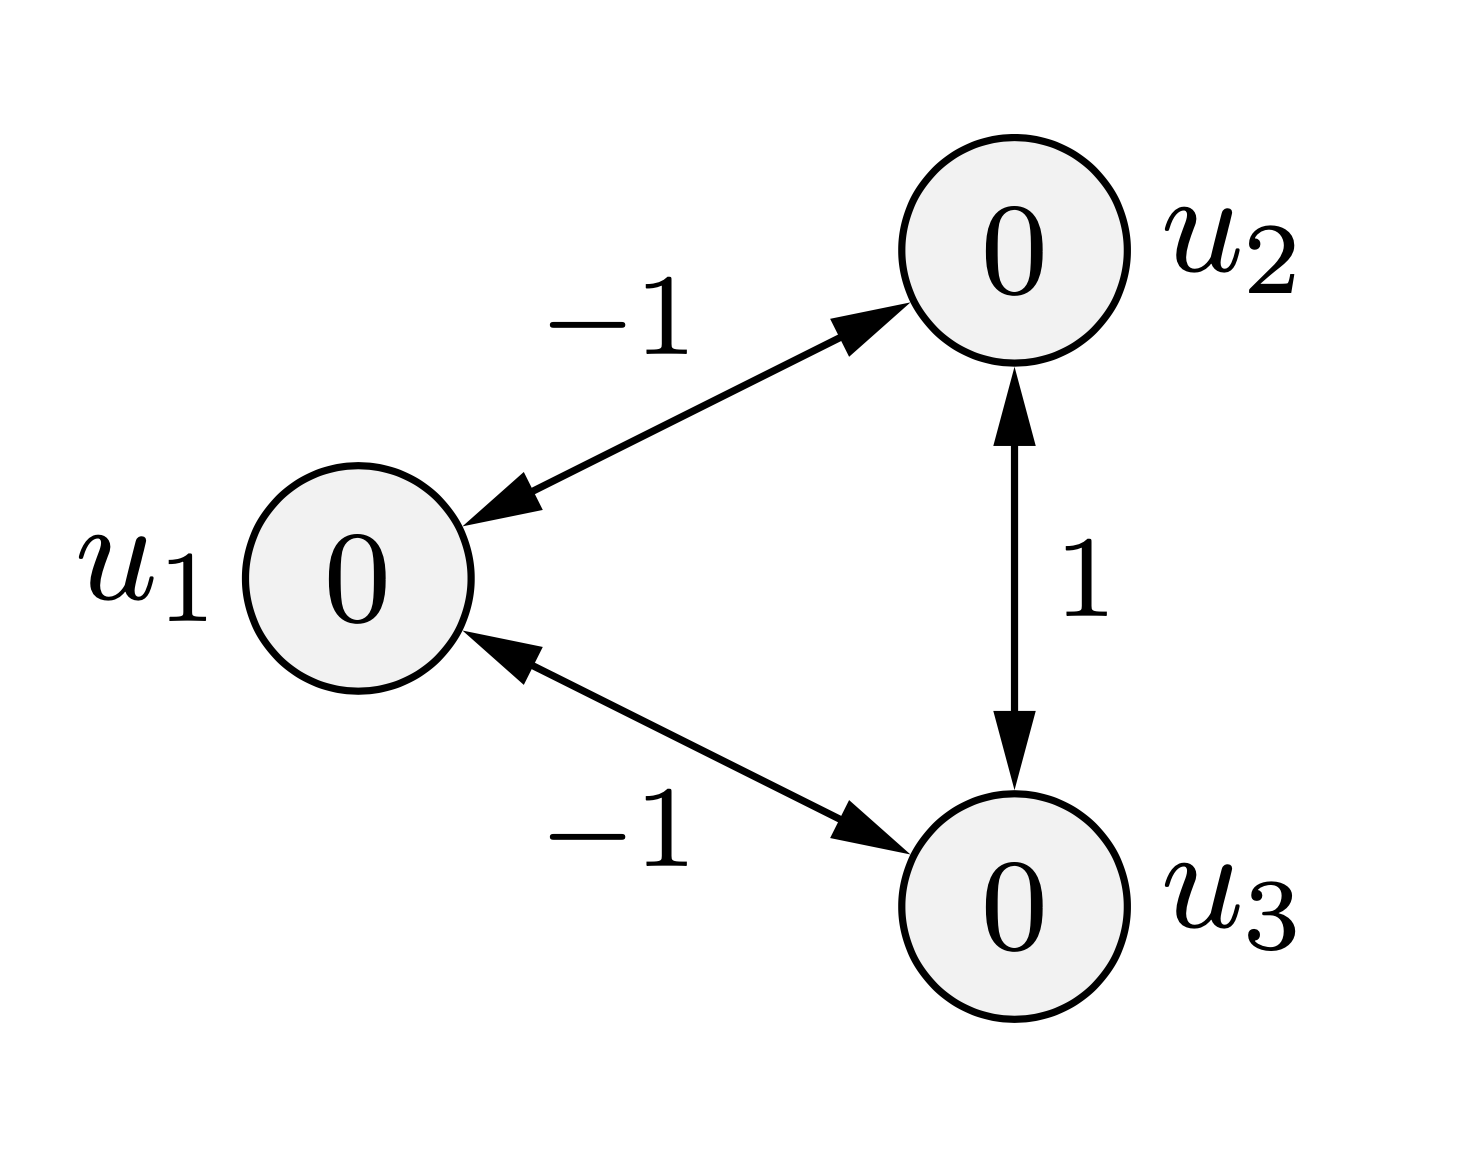
\includegraphics[width=.2\textwidth]{im1.png}
        \hfil
    \end{floatingfigure}
    Determine the energy function of the Hopfield network of Exercise 45! With the help of this energy function, compute the energies of the individual states of the network. Then arrange the states according to their energy, that is, draw a new state transition graph, in which the location of the states indicates their energy!\par\medskip
    The energy function of a Hopfield network:
    \[
        E=-\frac12\vec{act}^\top{\bf{W}} \vec{act}+\underbrace{\vec\theta^\top\vec{act}}_0 \qquad \text{(from lesson)}
    \]

    % Горизонтальная линия
    \bigskip
    \hrule width 3cm height 1pt
    \vskip 1pt \hrule width 3cm
    \medskip\par\smallskip

    \begin{center}  
        \large
        \textbf{Solution}
    \end{center}

    \[
        {\bf W}=
        \begin{pmatrix}
            0 & -1 & -1\\
            -1 & 0 & 1\\
            -1 & 1 & 0\\
        \end{pmatrix}
    \]\par

    $
    \vec{act}=(-1, -1, -1)^\top\Rightarrow E(---)=1;\\
    \vec{act}=(+1, -1, -1)^\top\Rightarrow E(+--)=-3;\\
    $
    \par\bigskip

    \begin{figure}[h]
        \centering
        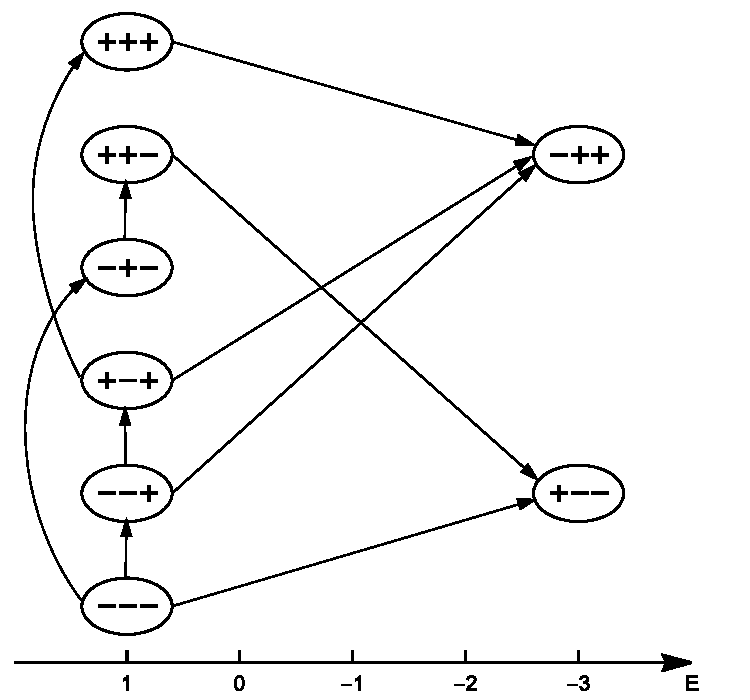
\includegraphics[width=90mm]{im5.pdf}
    \end{figure}

\newpage

\blindtext

\end{document}


